% Created by tikzDevice version 0.10.1 on 2018-01-24 12:51:54
% !TEX encoding = UTF-8 Unicode
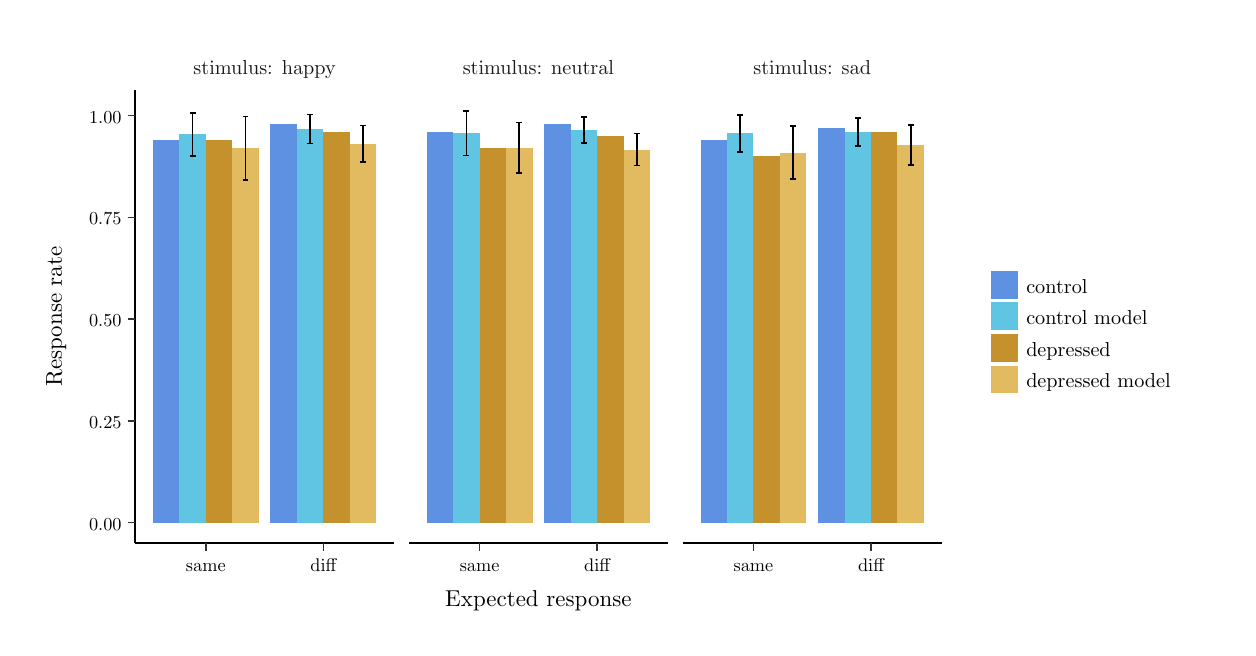
\begin{tikzpicture}[x=1pt,y=1pt]
\definecolor{fillColor}{RGB}{255,255,255}
\path[use as bounding box,fill=fillColor,fill opacity=0.00] (0,0) rectangle (433.62,216.81);
\begin{scope}
\path[clip] (  0.00,  0.00) rectangle (433.62,216.81);
\definecolor{drawColor}{RGB}{255,255,255}
\definecolor{fillColor}{RGB}{255,255,255}

\path[draw=drawColor,line width= 0.6pt,line join=round,line cap=round,fill=fillColor] (  0.00,  0.00) rectangle (433.62,216.81);
\end{scope}
\begin{scope}
\path[clip] ( 38.88, 30.56) rectangle (132.33,194.25);
\definecolor{fillColor}{RGB}{255,255,255}

\path[fill=fillColor] ( 38.88, 30.56) rectangle (132.33,194.25);
\definecolor{fillColor}{RGB}{226,186,95}

\path[fill=fillColor] ( 73.93, 38.00) rectangle ( 83.48,173.23);
\definecolor{fillColor}{RGB}{196,145,45}

\path[fill=fillColor] ( 64.37, 38.00) rectangle ( 73.93,176.19);
\definecolor{fillColor}{RGB}{95,197,226}

\path[fill=fillColor] ( 54.81, 38.00) rectangle ( 64.37,178.27);
\definecolor{fillColor}{RGB}{95,145,226}

\path[fill=fillColor] ( 45.26, 38.00) rectangle ( 54.81,176.19);
\definecolor{fillColor}{RGB}{226,186,95}

\path[fill=fillColor] (116.40, 38.00) rectangle (125.96,174.86);
\definecolor{fillColor}{RGB}{196,145,45}

\path[fill=fillColor] (106.84, 38.00) rectangle (116.40,179.13);
\definecolor{fillColor}{RGB}{95,197,226}

\path[fill=fillColor] ( 97.29, 38.00) rectangle (106.84,180.14);
\definecolor{fillColor}{RGB}{95,145,226}

\path[fill=fillColor] ( 87.73, 38.00) rectangle ( 97.29,182.07);
\definecolor{drawColor}{RGB}{0,0,0}

\path[draw=drawColor,line width= 0.6pt,line join=round] ( 77.64,184.68) --
	( 79.77,184.68);

\path[draw=drawColor,line width= 0.6pt,line join=round] ( 78.70,184.68) --
	( 78.70,161.78);

\path[draw=drawColor,line width= 0.6pt,line join=round] ( 77.64,161.78) --
	( 79.77,161.78);

\path[draw=drawColor,line width= 0.6pt,line join=round] ( 58.53,186.07) --
	( 60.65,186.07);

\path[draw=drawColor,line width= 0.6pt,line join=round] ( 59.59,186.07) --
	( 59.59,170.48);

\path[draw=drawColor,line width= 0.6pt,line join=round] ( 58.53,170.48) --
	( 60.65,170.48);

\path[draw=drawColor,line width= 0.6pt,line join=round] (120.12,181.43) --
	(122.24,181.43);

\path[draw=drawColor,line width= 0.6pt,line join=round] (121.18,181.43) --
	(121.18,168.29);

\path[draw=drawColor,line width= 0.6pt,line join=round] (120.12,168.29) --
	(122.24,168.29);

\path[draw=drawColor,line width= 0.6pt,line join=round] (101.00,185.38) --
	(103.13,185.38);

\path[draw=drawColor,line width= 0.6pt,line join=round] (102.07,185.38) --
	(102.07,174.90);

\path[draw=drawColor,line width= 0.6pt,line join=round] (101.00,174.90) --
	(103.13,174.90);
\end{scope}
\begin{scope}
\path[clip] (137.83, 30.56) rectangle (231.27,194.25);
\definecolor{fillColor}{RGB}{255,255,255}

\path[fill=fillColor] (137.83, 30.56) rectangle (231.27,194.25);
\definecolor{fillColor}{RGB}{226,186,95}

\path[fill=fillColor] (172.87, 38.00) rectangle (182.43,173.38);
\definecolor{fillColor}{RGB}{196,145,45}

\path[fill=fillColor] (163.31, 38.00) rectangle (172.87,173.24);
\definecolor{fillColor}{RGB}{95,197,226}

\path[fill=fillColor] (153.76, 38.00) rectangle (163.31,178.74);
\definecolor{fillColor}{RGB}{95,145,226}

\path[fill=fillColor] (144.20, 38.00) rectangle (153.76,179.13);
\definecolor{fillColor}{RGB}{226,186,95}

\path[fill=fillColor] (215.34, 38.00) rectangle (224.90,172.75);
\definecolor{fillColor}{RGB}{196,145,45}

\path[fill=fillColor] (205.79, 38.00) rectangle (215.34,177.66);
\definecolor{fillColor}{RGB}{95,197,226}

\path[fill=fillColor] (196.23, 38.00) rectangle (205.79,179.88);
\definecolor{fillColor}{RGB}{95,145,226}

\path[fill=fillColor] (186.67, 38.00) rectangle (196.23,182.07);
\definecolor{drawColor}{RGB}{0,0,0}

\path[draw=drawColor,line width= 0.6pt,line join=round] (176.59,182.52) --
	(178.71,182.52);

\path[draw=drawColor,line width= 0.6pt,line join=round] (177.65,182.52) --
	(177.65,164.24);

\path[draw=drawColor,line width= 0.6pt,line join=round] (176.59,164.24) --
	(178.71,164.24);

\path[draw=drawColor,line width= 0.6pt,line join=round] (157.47,186.81) --
	(159.60,186.81);

\path[draw=drawColor,line width= 0.6pt,line join=round] (158.53,186.81) --
	(158.53,170.67);

\path[draw=drawColor,line width= 0.6pt,line join=round] (157.47,170.67) --
	(159.60,170.67);

\path[draw=drawColor,line width= 0.6pt,line join=round] (219.06,178.52) --
	(221.18,178.52);

\path[draw=drawColor,line width= 0.6pt,line join=round] (220.12,178.52) --
	(220.12,166.98);

\path[draw=drawColor,line width= 0.6pt,line join=round] (219.06,166.98) --
	(221.18,166.98);

\path[draw=drawColor,line width= 0.6pt,line join=round] (199.95,184.64) --
	(202.07,184.64);

\path[draw=drawColor,line width= 0.6pt,line join=round] (201.01,184.64) --
	(201.01,175.12);

\path[draw=drawColor,line width= 0.6pt,line join=round] (199.95,175.12) --
	(202.07,175.12);
\end{scope}
\begin{scope}
\path[clip] (236.77, 30.56) rectangle (330.22,194.25);
\definecolor{fillColor}{RGB}{255,255,255}

\path[fill=fillColor] (236.77, 30.56) rectangle (330.22,194.25);
\definecolor{fillColor}{RGB}{226,186,95}

\path[fill=fillColor] (271.81, 38.00) rectangle (281.37,171.67);
\definecolor{fillColor}{RGB}{196,145,45}

\path[fill=fillColor] (262.26, 38.00) rectangle (271.81,170.30);
\definecolor{fillColor}{RGB}{95,197,226}

\path[fill=fillColor] (252.70, 38.00) rectangle (262.26,178.62);
\definecolor{fillColor}{RGB}{95,145,226}

\path[fill=fillColor] (243.14, 38.00) rectangle (252.70,176.19);
\definecolor{fillColor}{RGB}{226,186,95}

\path[fill=fillColor] (314.29, 38.00) rectangle (323.85,174.34);
\definecolor{fillColor}{RGB}{196,145,45}

\path[fill=fillColor] (304.73, 38.00) rectangle (314.29,179.13);
\definecolor{fillColor}{RGB}{95,197,226}

\path[fill=fillColor] (295.18, 38.00) rectangle (304.73,179.06);
\definecolor{fillColor}{RGB}{95,145,226}

\path[fill=fillColor] (285.62, 38.00) rectangle (295.18,180.60);
\definecolor{drawColor}{RGB}{0,0,0}

\path[draw=drawColor,line width= 0.6pt,line join=round] (275.53,181.30) --
	(277.65,181.30);

\path[draw=drawColor,line width= 0.6pt,line join=round] (276.59,181.30) --
	(276.59,162.05);

\path[draw=drawColor,line width= 0.6pt,line join=round] (275.53,162.05) --
	(277.65,162.05);

\path[draw=drawColor,line width= 0.6pt,line join=round] (256.42,185.32) --
	(258.54,185.32);

\path[draw=drawColor,line width= 0.6pt,line join=round] (257.48,185.32) --
	(257.48,171.91);

\path[draw=drawColor,line width= 0.6pt,line join=round] (256.42,171.91) --
	(258.54,171.91);

\path[draw=drawColor,line width= 0.6pt,line join=round] (318.01,181.56) --
	(320.13,181.56);

\path[draw=drawColor,line width= 0.6pt,line join=round] (319.07,181.56) --
	(319.07,167.11);

\path[draw=drawColor,line width= 0.6pt,line join=round] (318.01,167.11) --
	(320.13,167.11);

\path[draw=drawColor,line width= 0.6pt,line join=round] (298.89,184.11) --
	(301.02,184.11);

\path[draw=drawColor,line width= 0.6pt,line join=round] (299.95,184.11) --
	(299.95,174.01);

\path[draw=drawColor,line width= 0.6pt,line join=round] (298.89,174.01) --
	(301.02,174.01);
\end{scope}
\begin{scope}
\path[clip] ( 38.88,194.25) rectangle (132.33,211.31);
\definecolor{drawColor}{RGB}{255,255,255}
\definecolor{fillColor}{RGB}{255,255,255}

\path[draw=drawColor,line width= 1.1pt,line join=round,line cap=round,fill=fillColor] ( 38.88,194.25) rectangle (132.33,211.31);
\definecolor{drawColor}{gray}{0.10}

\node[text=drawColor,anchor=base,inner sep=0pt, outer sep=0pt, scale=  0.73] at ( 85.61,199.75) {stimulus: happy};
\end{scope}
\begin{scope}
\path[clip] (137.83,194.25) rectangle (231.27,211.31);
\definecolor{drawColor}{RGB}{255,255,255}
\definecolor{fillColor}{RGB}{255,255,255}

\path[draw=drawColor,line width= 1.1pt,line join=round,line cap=round,fill=fillColor] (137.83,194.25) rectangle (231.27,211.31);
\definecolor{drawColor}{gray}{0.10}

\node[text=drawColor,anchor=base,inner sep=0pt, outer sep=0pt, scale=  0.73] at (184.55,199.75) {stimulus: neutral};
\end{scope}
\begin{scope}
\path[clip] (236.77,194.25) rectangle (330.22,211.31);
\definecolor{drawColor}{RGB}{255,255,255}
\definecolor{fillColor}{RGB}{255,255,255}

\path[draw=drawColor,line width= 1.1pt,line join=round,line cap=round,fill=fillColor] (236.77,194.25) rectangle (330.22,211.31);
\definecolor{drawColor}{gray}{0.10}

\node[text=drawColor,anchor=base,inner sep=0pt, outer sep=0pt, scale=  0.73] at (283.49,199.75) {stimulus: sad};
\end{scope}
\begin{scope}
\path[clip] (  0.00,  0.00) rectangle (433.62,216.81);
\definecolor{drawColor}{RGB}{0,0,0}

\path[draw=drawColor,line width= 0.6pt,line join=round] ( 38.88, 30.56) --
	(132.33, 30.56);
\end{scope}
\begin{scope}
\path[clip] (  0.00,  0.00) rectangle (433.62,216.81);
\definecolor{drawColor}{gray}{0.20}

\path[draw=drawColor,line width= 0.6pt,line join=round] ( 64.37, 27.81) --
	( 64.37, 30.56);

\path[draw=drawColor,line width= 0.6pt,line join=round] (106.84, 27.81) --
	(106.84, 30.56);
\end{scope}
\begin{scope}
\path[clip] (  0.00,  0.00) rectangle (433.62,216.81);
\definecolor{drawColor}{RGB}{0,0,0}

\node[text=drawColor,anchor=base,inner sep=0pt, outer sep=0pt, scale=  0.66] at ( 64.37, 20.15) {same};

\node[text=drawColor,anchor=base,inner sep=0pt, outer sep=0pt, scale=  0.66] at (106.84, 20.15) {diff};
\end{scope}
\begin{scope}
\path[clip] (  0.00,  0.00) rectangle (433.62,216.81);
\definecolor{drawColor}{RGB}{0,0,0}

\path[draw=drawColor,line width= 0.6pt,line join=round] (137.83, 30.56) --
	(231.27, 30.56);
\end{scope}
\begin{scope}
\path[clip] (  0.00,  0.00) rectangle (433.62,216.81);
\definecolor{drawColor}{gray}{0.20}

\path[draw=drawColor,line width= 0.6pt,line join=round] (163.31, 27.81) --
	(163.31, 30.56);

\path[draw=drawColor,line width= 0.6pt,line join=round] (205.79, 27.81) --
	(205.79, 30.56);
\end{scope}
\begin{scope}
\path[clip] (  0.00,  0.00) rectangle (433.62,216.81);
\definecolor{drawColor}{RGB}{0,0,0}

\node[text=drawColor,anchor=base,inner sep=0pt, outer sep=0pt, scale=  0.66] at (163.31, 20.15) {same};

\node[text=drawColor,anchor=base,inner sep=0pt, outer sep=0pt, scale=  0.66] at (205.79, 20.15) {diff};
\end{scope}
\begin{scope}
\path[clip] (  0.00,  0.00) rectangle (433.62,216.81);
\definecolor{drawColor}{RGB}{0,0,0}

\path[draw=drawColor,line width= 0.6pt,line join=round] (236.77, 30.56) --
	(330.22, 30.56);
\end{scope}
\begin{scope}
\path[clip] (  0.00,  0.00) rectangle (433.62,216.81);
\definecolor{drawColor}{gray}{0.20}

\path[draw=drawColor,line width= 0.6pt,line join=round] (262.26, 27.81) --
	(262.26, 30.56);

\path[draw=drawColor,line width= 0.6pt,line join=round] (304.73, 27.81) --
	(304.73, 30.56);
\end{scope}
\begin{scope}
\path[clip] (  0.00,  0.00) rectangle (433.62,216.81);
\definecolor{drawColor}{RGB}{0,0,0}

\node[text=drawColor,anchor=base,inner sep=0pt, outer sep=0pt, scale=  0.66] at (262.26, 20.15) {same};

\node[text=drawColor,anchor=base,inner sep=0pt, outer sep=0pt, scale=  0.66] at (304.73, 20.15) {diff};
\end{scope}
\begin{scope}
\path[clip] (  0.00,  0.00) rectangle (433.62,216.81);
\definecolor{drawColor}{RGB}{0,0,0}

\path[draw=drawColor,line width= 0.6pt,line join=round] ( 38.88, 30.56) --
	( 38.88,194.25);
\end{scope}
\begin{scope}
\path[clip] (  0.00,  0.00) rectangle (433.62,216.81);
\definecolor{drawColor}{RGB}{0,0,0}

\node[text=drawColor,anchor=base east,inner sep=0pt, outer sep=0pt, scale=  0.66] at ( 33.93, 35.27) {0.00};

\node[text=drawColor,anchor=base east,inner sep=0pt, outer sep=0pt, scale=  0.66] at ( 33.93, 72.02) {0.25};

\node[text=drawColor,anchor=base east,inner sep=0pt, outer sep=0pt, scale=  0.66] at ( 33.93,108.77) {0.50};

\node[text=drawColor,anchor=base east,inner sep=0pt, outer sep=0pt, scale=  0.66] at ( 33.93,145.53) {0.75};

\node[text=drawColor,anchor=base east,inner sep=0pt, outer sep=0pt, scale=  0.66] at ( 33.93,182.28) {1.00};
\end{scope}
\begin{scope}
\path[clip] (  0.00,  0.00) rectangle (433.62,216.81);
\definecolor{drawColor}{gray}{0.20}

\path[draw=drawColor,line width= 0.6pt,line join=round] ( 36.13, 38.00) --
	( 38.88, 38.00);

\path[draw=drawColor,line width= 0.6pt,line join=round] ( 36.13, 74.75) --
	( 38.88, 74.75);

\path[draw=drawColor,line width= 0.6pt,line join=round] ( 36.13,111.50) --
	( 38.88,111.50);

\path[draw=drawColor,line width= 0.6pt,line join=round] ( 36.13,148.25) --
	( 38.88,148.25);

\path[draw=drawColor,line width= 0.6pt,line join=round] ( 36.13,185.01) --
	( 38.88,185.01);
\end{scope}
\begin{scope}
\path[clip] (  0.00,  0.00) rectangle (433.62,216.81);
\definecolor{drawColor}{RGB}{0,0,0}

\node[text=drawColor,anchor=base,inner sep=0pt, outer sep=0pt, scale=  0.83] at (184.55,  7.83) {Expected response};
\end{scope}
\begin{scope}
\path[clip] (  0.00,  0.00) rectangle (433.62,216.81);
\definecolor{drawColor}{RGB}{0,0,0}

\node[text=drawColor,rotate= 90.00,anchor=base,inner sep=0pt, outer sep=0pt, scale=  0.83] at ( 12.32,112.40) {Response rate};
\end{scope}
\begin{scope}
\path[clip] (  0.00,  0.00) rectangle (433.62,216.81);
\definecolor{fillColor}{RGB}{255,255,255}

\path[fill=fillColor] (341.60, 78.37) rectangle (428.12,146.43);
\end{scope}
\begin{scope}
\path[clip] (  0.00,  0.00) rectangle (433.62,216.81);
\definecolor{fillColor}{RGB}{95,145,226}

\path[fill=fillColor] (348.00,118.92) rectangle (357.96,128.88);
\end{scope}
\begin{scope}
\path[clip] (  0.00,  0.00) rectangle (433.62,216.81);
\definecolor{fillColor}{RGB}{95,197,226}

\path[fill=fillColor] (348.00,107.54) rectangle (357.96,117.50);
\end{scope}
\begin{scope}
\path[clip] (  0.00,  0.00) rectangle (433.62,216.81);
\definecolor{fillColor}{RGB}{196,145,45}

\path[fill=fillColor] (348.00, 96.16) rectangle (357.96,106.11);
\end{scope}
\begin{scope}
\path[clip] (  0.00,  0.00) rectangle (433.62,216.81);
\definecolor{fillColor}{RGB}{226,186,95}

\path[fill=fillColor] (348.00, 84.77) rectangle (357.96, 94.73);
\end{scope}
\begin{scope}
\path[clip] (  0.00,  0.00) rectangle (433.62,216.81);
\definecolor{drawColor}{RGB}{0,0,0}

\node[text=drawColor,anchor=base west,inner sep=0pt, outer sep=0pt, scale=  0.73] at (360.84,120.87) {control};
\end{scope}
\begin{scope}
\path[clip] (  0.00,  0.00) rectangle (433.62,216.81);
\definecolor{drawColor}{RGB}{0,0,0}

\node[text=drawColor,anchor=base west,inner sep=0pt, outer sep=0pt, scale=  0.73] at (360.84,109.49) {control model};
\end{scope}
\begin{scope}
\path[clip] (  0.00,  0.00) rectangle (433.62,216.81);
\definecolor{drawColor}{RGB}{0,0,0}

\node[text=drawColor,anchor=base west,inner sep=0pt, outer sep=0pt, scale=  0.73] at (360.84, 98.10) {depressed};
\end{scope}
\begin{scope}
\path[clip] (  0.00,  0.00) rectangle (433.62,216.81);
\definecolor{drawColor}{RGB}{0,0,0}

\node[text=drawColor,anchor=base west,inner sep=0pt, outer sep=0pt, scale=  0.73] at (360.84, 86.72) {depressed model};
\end{scope}
\end{tikzpicture}
